\documentclass[11pt,a4paper]{article}

\usepackage[english]{babel}
\usepackage[T1]{fontenc}
\usepackage[utf8]{inputenc}
\usepackage{graphicx}
\graphicspath{{../Figs/}}
\usepackage{float}
\usepackage[font=footnotesize,labelfont={sf,bf},textfont=sf,width=\textwidth]{caption}
\usepackage[margin=2cm]{geometry}
\usepackage[plainpages=false,pdfpagelabels,hypertexnames=false,hidelinks]{hyperref}
\usepackage[usenames,dvipsnames]{xcolor}
\usepackage{mathtools}
\usepackage{siunitx}
\usepackage{booktabs}
%\usepackage{amsmath}
%\usepackage{amssymb}
%\usepackage{amsthm}


\title{\bfseries\textsc{Measurement of Cotton-Mouton effect}}
\author{
Michele Masini\\ \small\texttt{\href{mailto:michele.masini@uni-ulm.de}{michele.masini@uni-ulm.de}}\and
Iyán Méndez Veiga\\ \small\texttt{\href{mailto:iyan.mendez-veiga@uni-ulm.de}{iyan.mendez-veiga@uni-ulm.de}}
}
\date{\today}


\begin{document}
\maketitle

\begin{abstract}
In the following report, we will describe the procedure for the measurement of the Cotton-Mouton effect in three materials: carbon disulfide, mesitylene and toluene. Firstly, we measured the proportionality with the current and the uniformity of the magnetic field used to realize the Cotton-Mouton effect. Secondly, we checked the linearity of the Faraday effect used to rotate the polarization of light in our experiment. Finally, we measured the Cotton-Mouton effect minimizing the intensity of the beam of a laser by means of the Faraday effect.
\end{abstract}

\vspace{1.5cm}

\section{Introduction}

{\color{red}What? and Why? not theory here}

\vspace{.5cm}

With magneto-optic effects, one means those effects that change properties of light when it passes through a material in presence of a magnetic field applied.	There are two well-known magneto-optic effects: the Faraday effect and Cotton-Mouton effect.
	
The former occurs when we apply a magnetic field to a material in the same direction of the propagation of light. We will have a rotation ($\theta_F$) of the plane of vibration of the electromagnetic wave. Let $\phi$ be the angle between $\vec{B}$ and the propagation of light, $l$ the thickness of the sample, $B$ the absolute value of the magnetic field, then

\begin{equation}
\theta_F=lBVcos\phi
\end{equation}
where $V$ is called Verdet constant \cite{cappelli2003cotton}. 

Besides this first order effect, it is possible to measure also a second order one: the Cotton-Mouton effect. This is the one that we will measure in our experiment. It stimulates a birefringence in the material where the magnetic field is applied, i.e. refractive indices which depend on the polarization of light. Usually, we refer to birefringence as the difference between the maximum and the minimum refractive index in the material: $\Delta n=n_{max}-n_{min}$.

Thanks to the latter effect, the electromagnetic wave will have a phase difference $\delta=\frac{2\pi \Delta n L}{\lambda}$ where $L$ is the optical path. It is possible to express the phase difference in dependence of the magnetic field:

\begin{equation}
\delta=C2\pi L B^2
\end{equation}
where $C=C(\lambda,T)$ is the \emph{Cotton-Mouton constant} \cite{wilson1997simple}.
	
In our experiment, we had the following steps:

\begin{enumerate}
\item The beam of a laser passes through a polarizer in order to obtain linear polarization.
\item By means of Faraday effect (the magnetic field is produced with a solenoid) the direction of the polarization is rotated.
\item A quarter wave-plate set in the same direction of the polarizer produces elliptical polarization if the magnetic effect in the previous step rotates the polarization
\item We stimulate a birefringence using the Cotton-Mouton effect. A magnetic field is applied to a sample
\item The beam passes through an analyzer
\item We measure the intensity of the beam by means of a photodiode and a lock-in amplifier
\end{enumerate}	

Firstly, we minimized the intensity of light skipping step 2. and 4., hence without magnetic fields.  The quarter wave-plate does not provide an elliptical polarization because it has the same direction of the polarizer in the first step; setting the analyzer we look for the angle that minimizes the gain of the photodiode. After this first step, the angles of the analyzer, polarizer and quarter wave-plate are left invariant for all the experiment.

Secondly, we insert the sample of step 4. and we apply a magnetic field through it. The Cotton-Mouton effect will produce a retard in the circular polarization. 

Finally, we look for the value of the intensity applied to the solenoid in step 3. that minimizes the gain of the photodiode. 

Let us now calculate the effect of the path using Jones matrices. bla bla bla calculation of the matrix bla bla bla

\section{Materials and methods}\label{mm}
In the first part of the experiment, we measured the proportionality of the magnetic field used to produce the Cotton-Mouton effect in step 4. with a Hall probe. The magnetic field was produced by means of a Helmholtz coil in order to make it as much uniform as possible. According to the Ampère law, the magnetic field can be expressed as:

\begin{equation}
B(I)=\frac{LI}{A}
\end{equation}
where $L$ is the inductance of the coil, $A$ is the surface and $I$ is the current flowing in the coil. In this part, we looked for the region of linearity of the magnetic field in function of the current $I$. The probe was positioned in the middle of the coils; we took a measurement of the magnetic field by changing the current at steps of $1mA$ from $-20mA$ to $+20mA$.

Secondly, we checked the uniformity of the magnetic field inside the coils in order to position the sample in the region where $\vec{B}$ is uniform. We took the measurements for 3 different values of the current flowing in the coil; the Helmholtz probe was moved at steps of $5mm$.

Thirdly, we verified the linearity of the Faraday effect. The beam of the laser passed respectively through the polarizer, the solenoid of step 2., the analyzer and ended in the photodiode. The solenoid was set in such a way that the magnetic field was parallel to the direction of the laser. Varying the intensity of the current applied to the solenoid we looked for the angle of the analyzer such that the gain of the photodiode was minimized.

The circuit used to produce Faraday effect was composed by a voltage generator, a solenoid and either 1 or 2 resistors. Using 2 resistors we will have less current at our disposal but more precision on the value of the intensity. On the countrary, using 1 reistor we will have higher intensities but less precision. We took measurements with both the configurations.

Finally, we measured Cotton-Mouton effect. The laser beam in this part used to follow all the steps described in section~\ref{mm}. During this part the magnetic field ($B_{CM}$) applied to one of the 3 samples was varied from $0mA$ to $10mA$. For every different $B_{CM}$ we looked for the value of the magnetic field ($B_F$) used to produce Faraday effect (step 2.) such that the gain of the photodiode was minimized.

\newpage

\section{Results and discussion}

\subsection{Characterising magnetic field}

We measured the magnetic field with the probe fixed in the middle for different values of current, first in one direction and then in the other.

\begin{figure}[H]
\centering
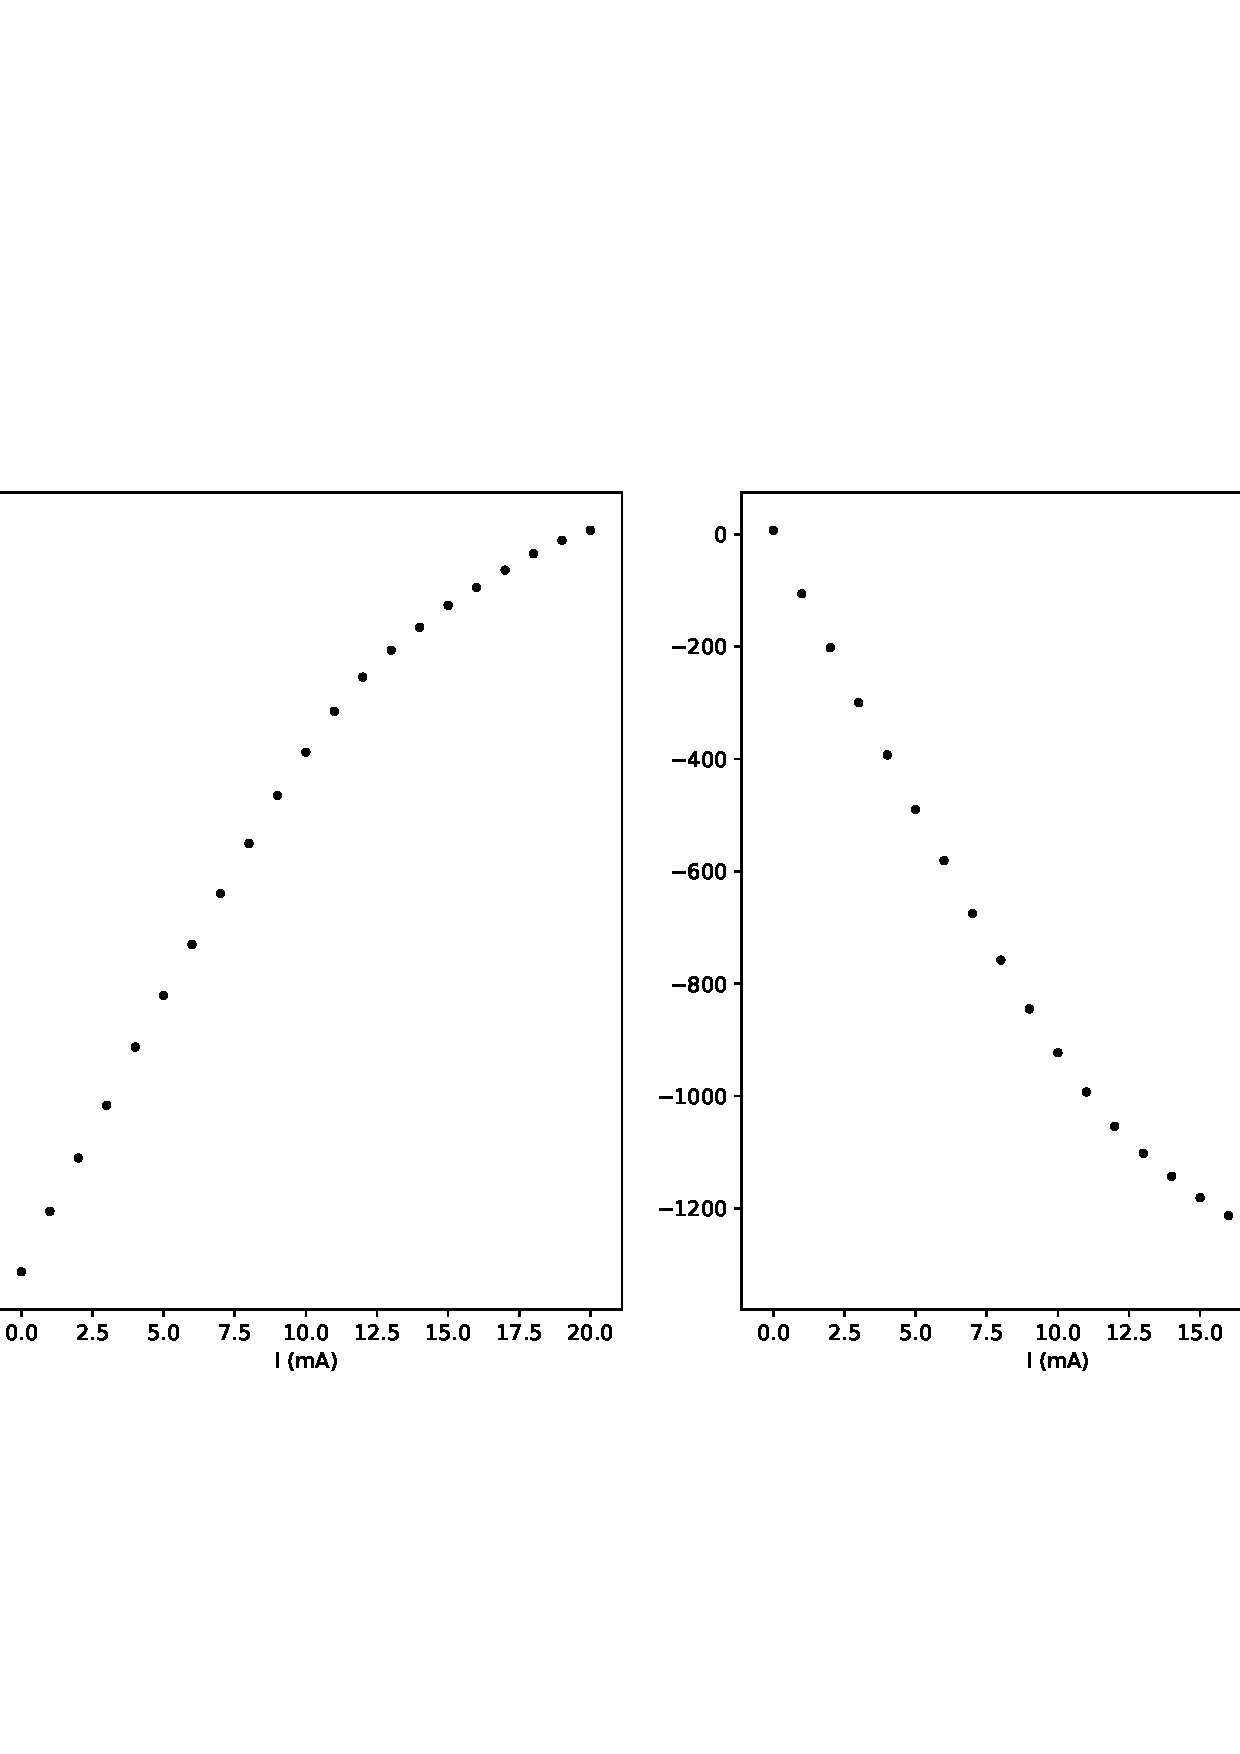
\includegraphics[width=0.9\textwidth]{B_diff_current.png}
\caption{Magnetic field as a function of current for the two circulating directions with the probe fixed in the middle of the solenoid.}
\label{fig:BvsI}
\end{figure}

Then we measured the magnetic field produced by a fixed current for different positions by moving the probe in steps of \SI{5}{\mm} from one end to the other. First measurement was done for a magnetic field produced by $I=\SI{10}{\mA}$.

\begin{figure}[H]
\centering
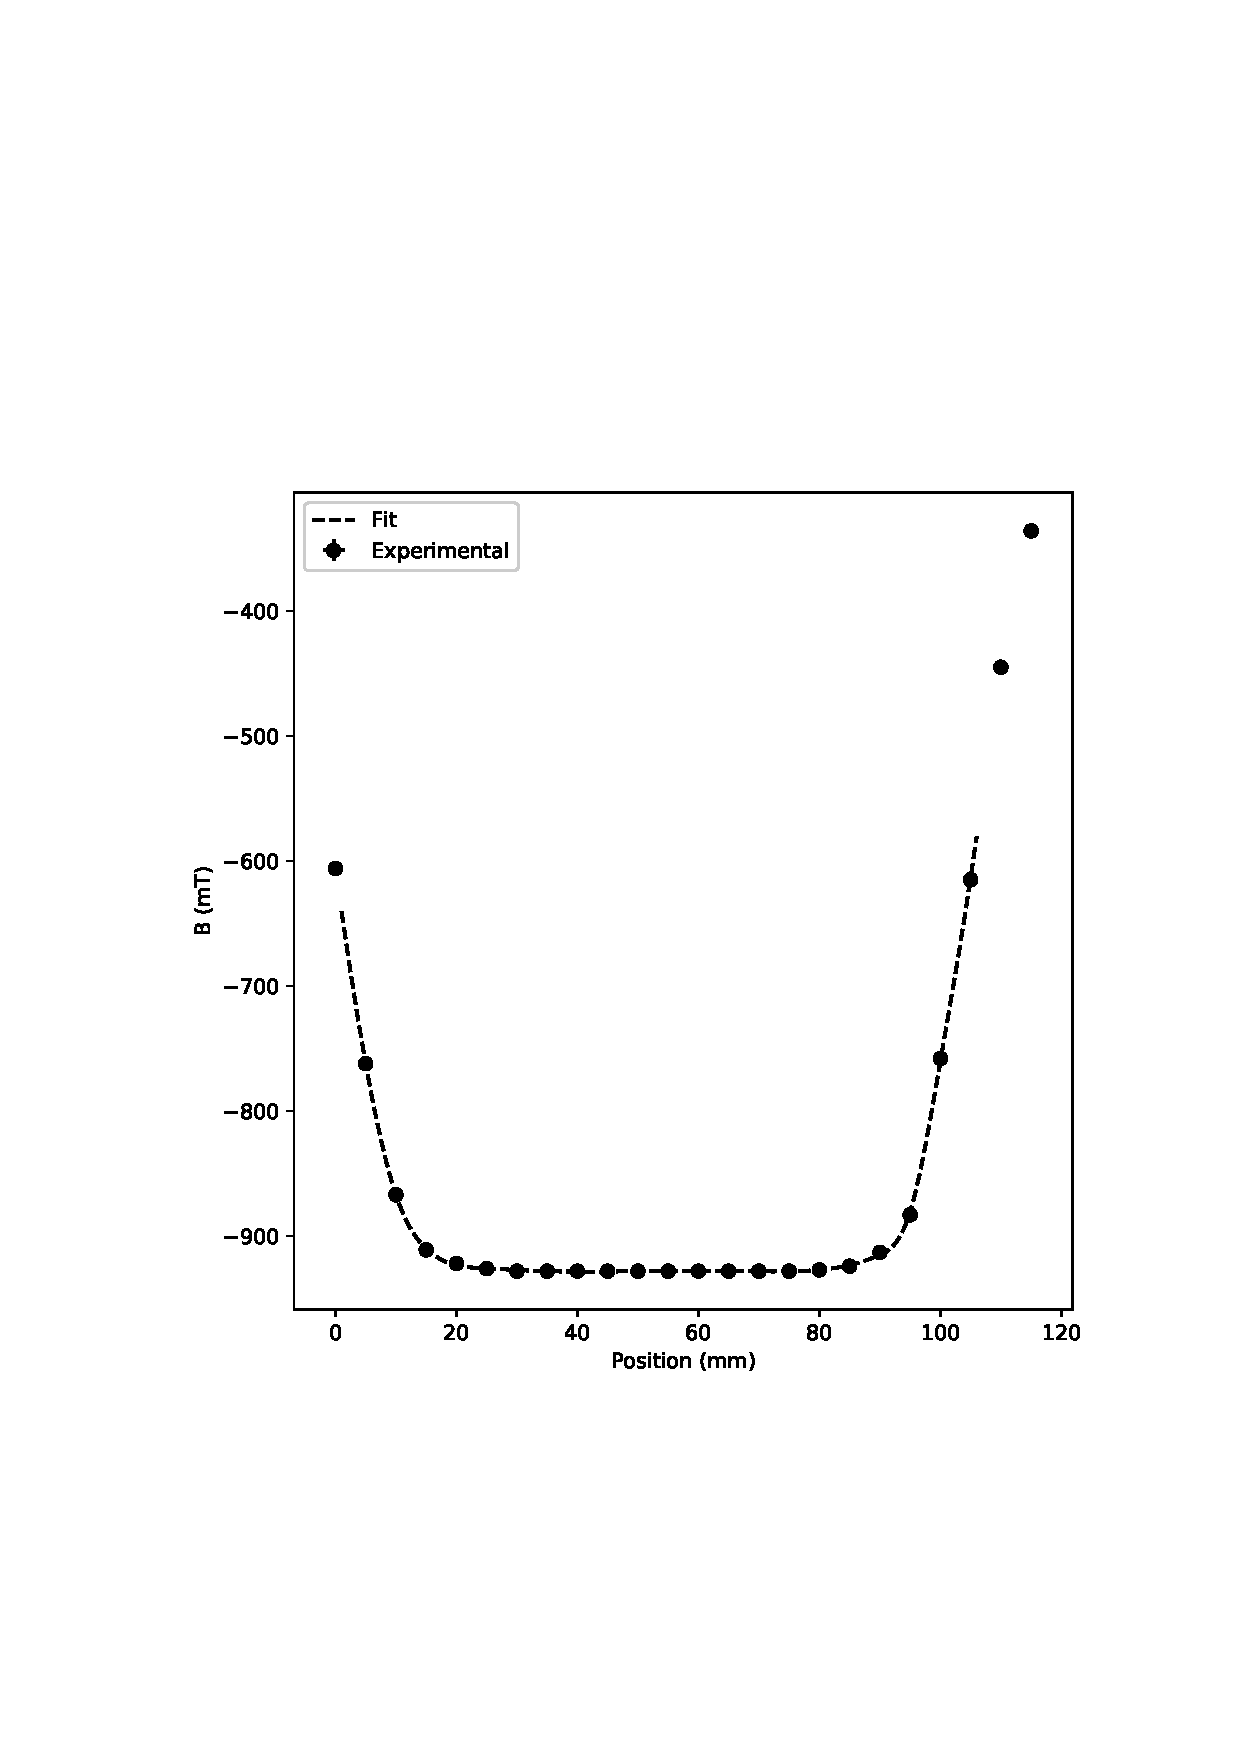
\includegraphics[width=0.55\textwidth]{B_diff_position1.png}
\caption{Magnetic field as a function of position for a fixed current of \SI{10}{\mA}.}
\label{fig:BvsPos1}
\end{figure}

Two more precise measurements due to a change of scale in the measuring device from \SI{2000}{mT} to \SI{20}{mT} were done later for a fixed value of current of $I=\SI{1}{\mA}$.

\begin{figure}[H]
\centering
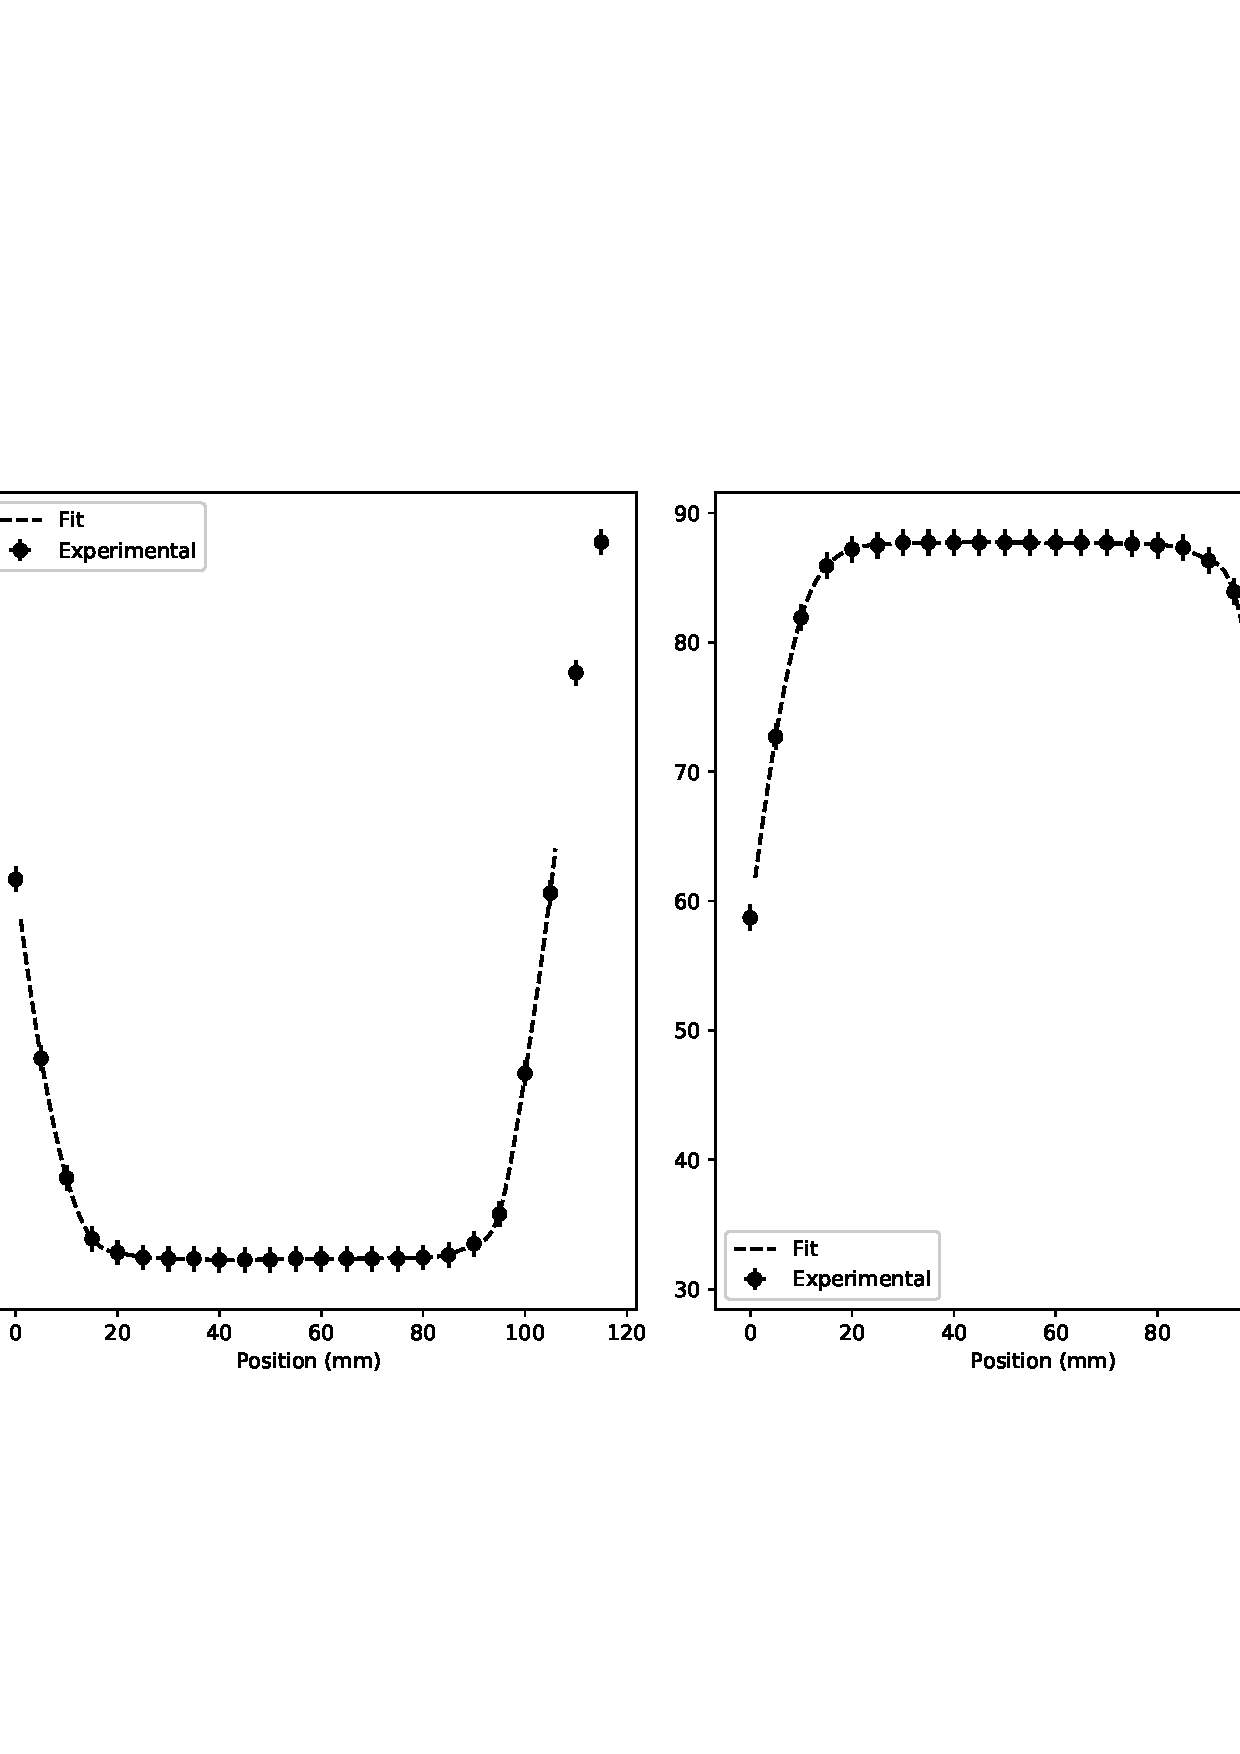
\includegraphics[width=0.9\textwidth]{B_diff_position2.png}
\caption{Magnetic field as a function of position for a fixed current of \SI{1}{\mA}. Direction of current was changed for each measurement.}
\label{fig:BvsPos2}
\end{figure}

\subsection{Determining Verdet constant}

We turned on the laser in order to measure the Faraday effect. For different values of current in the Faraday compensator (fig {\color{red}Add reference when photo is placed}), i.e. different values of the magnetic field in the direction of the propagation of the light, the angle of the analyser for which we minimised the signal at the detector was recorded. We repeated the measurements for both possible directions of the current and with one and two resistors.

Angles were measured in degrees, minutes and seconds using an optical device. These angles were processed into radians, the offset was subtracted and finally a linear regression was found using the method of least-squares (Figure \ref{fig:FaradayAngle}). The slope is precisely the modified Verdet constant of the Faraday compensator, which tells us how much the polarisation plane is rotated by the Faraday effect when applying a current of \SI{1}{mA}.

The following table summarises the values obtained for the Verded constant.

\begin{table}[H]
\centering
\begin{tabular}{ccc}
\toprule
Measurement & $V$ (\si{10^{-5}.\radian/\mA}) & $\delta V$ (\si{10^{-5}.\radian/\mA})\\
\midrule
2 resitors, pos 1 & -3.40 & 0.08 \\
1 resistor, pos 1 & -3.47 & 0.04 \\
2 resistors, pos 2 & -3.39 & 0.03 \\
1 resistors, pos 2 & -3.4 & 0.1 \\
\bottomrule
\end{tabular}
\caption{Values obtained for the modified Verdet constant with one and two resistors and for both directions of the current in the Faraday compensator.}
\label{table:verdet}
\end{table}

Uncertainties $\delta V$ were calculated by computing the square root of the covariances obtained from the least-squares fit.

\begin{figure}[H]
\centering
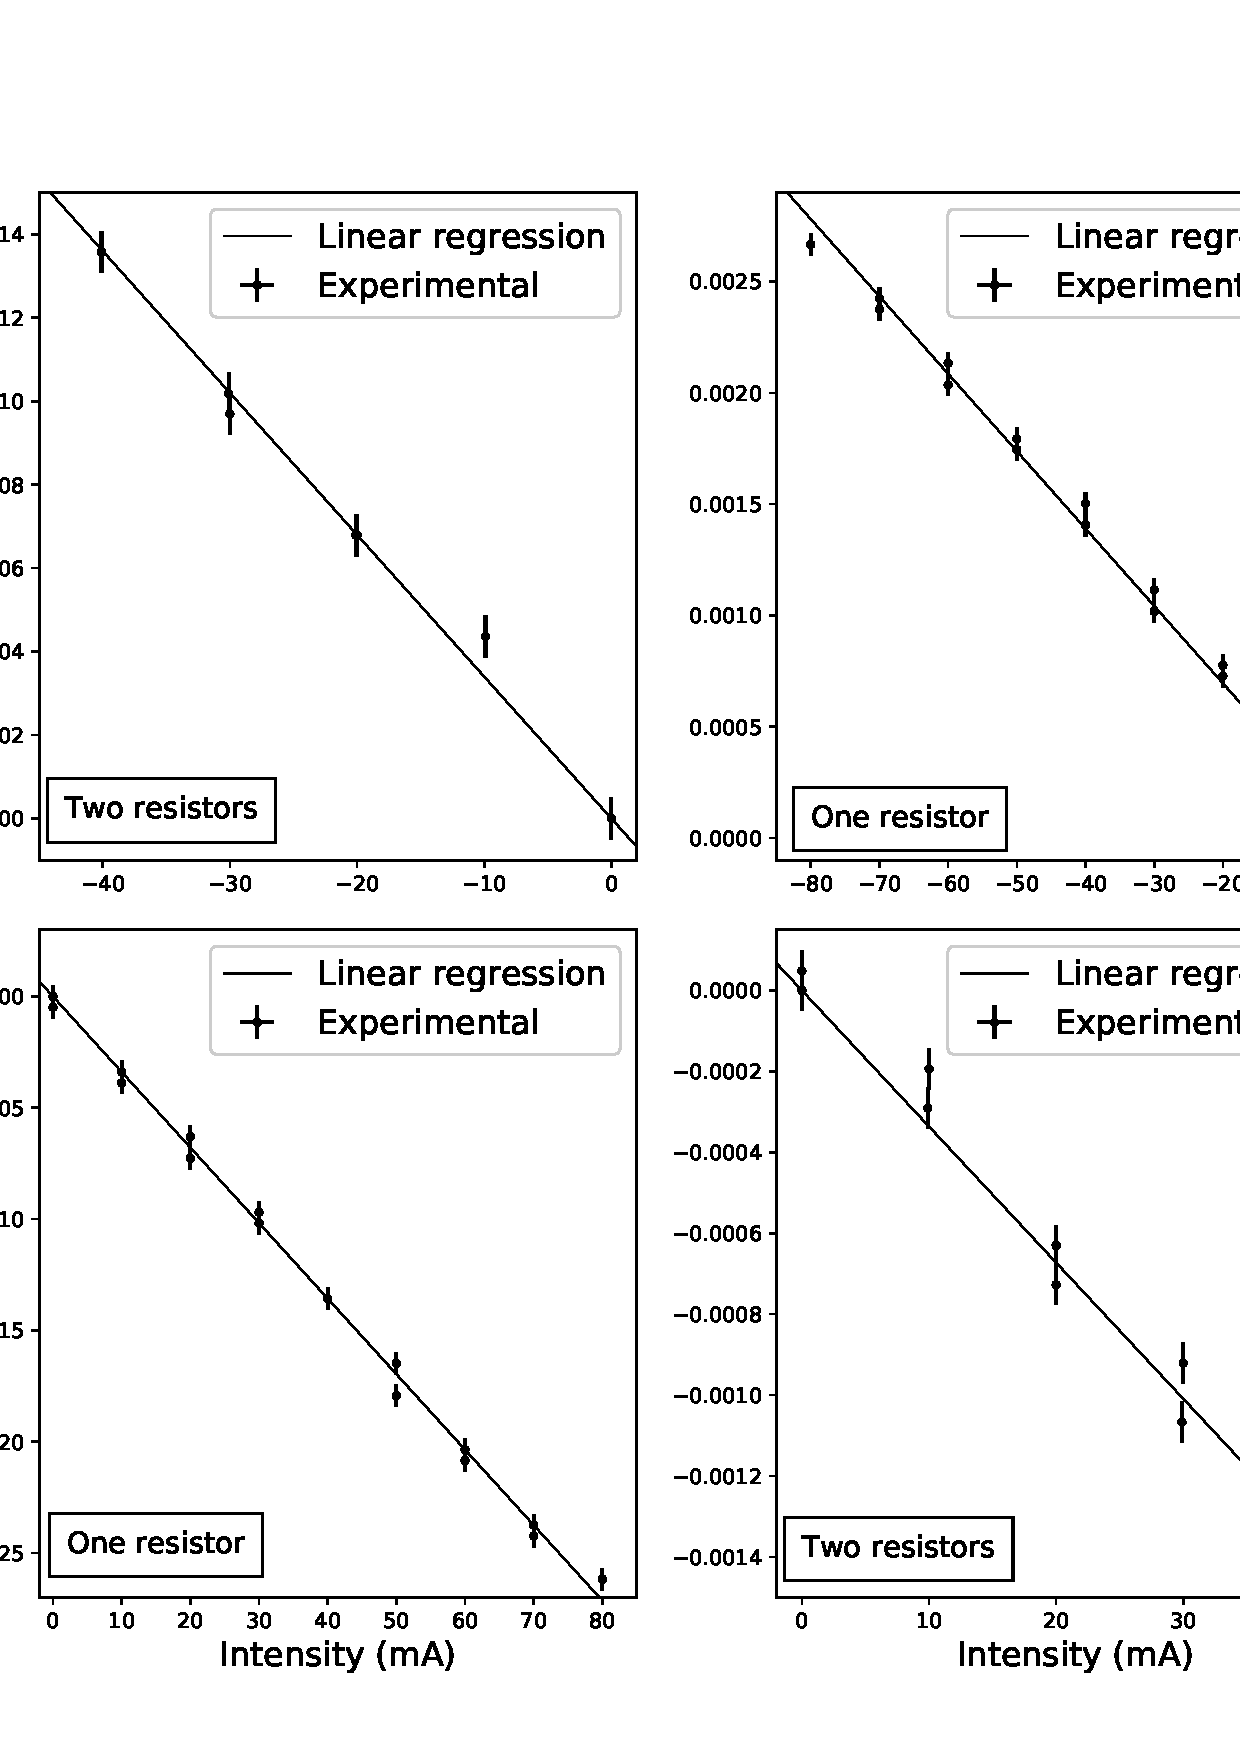
\includegraphics[width=\textwidth]{Angle_diff_intensity2.png}
\caption{Magnetic field as a function of position for a fixed current of \SI{1}{\mA}. Direction of current was changed for each measurement.}
\label{fig:FaradayAngle}
\end{figure}



\section{Conclusions}

\newpage
\bibliographystyle{unsrt}
\bibliography{references}


\end{document}